%%%%%%%%%%%%%%%%%%%%%%%%%%%%%%%%%%%%%%%%%
% University Assignment Title Page 
% LaTeX Template
% Version 1.0 (27/12/12)
%
% This template has been downloaded from:
% http://www.LaTeXTemplates.com
%
% Original author:
% WikiBooks (http://en.wikibooks.org/wiki/LaTeX/Title_Creation)
%
% License:
% CC BY-NC-SA 3.0 (http://creativecommons.org/licenses/by-nc-sa/3.0/)
% 
% Instructions for using this template:
% This title page is capable of being compiled as is. This is not useful for 
% including it in another document. To do this, you have two options: 
%
% 1) Copy/paste everything between \begin{document} and \end{document} 
% starting at \begin{titlepage} and paste this into another LaTeX file where you 
% want your title page.
% OR
% 2) Remove everything outside the \begin{titlepage} and \end{titlepage} and 
% move this file to the same directory as the LaTeX file you wish to add it to. 
% Then add \input{./title_page_1.tex} to your LaTeX file where you want your
% title page.
%
%%%%%%%%%%%%%%%%%%%%%%%%%%%%%%%%%%%%%%%%%

%----------------------------------------------------------------------------------------
%	PACKAGES AND OTHER DOCUMENT CONFIGURATIONS
%----------------------------------------------------------------------------------------

\documentclass[12pt]{article}
\usepackage[catalan]{babel}
\usepackage[utf8]{inputenc}
\usepackage{float}
\usepackage{graphicx}
\usepackage{wrapfig}
\usepackage{lscape}
\usepackage{rotating}
\usepackage{epstopdf}
\usepackage{makeidx}

\makeindex
\begin{document}
\begin{titlepage}

\newcommand{\HRule}{\rule{\linewidth}{0.5mm}} % Defines a new command for the horizontal lines, change thickness here

\center % Center everything on the page
 
%----------------------------------------------------------------------------------------
%	HEADING SECTIONS
%----------------------------------------------------------------------------------------

\textsc{\LARGE Universitat de Barcelona}\\[1.5cm] % Name of your university/college
\textsc{\Large Client-Servidor}\\[0.5cm] % Major heading such as course name
\textsc{\large Enfonsar la flota}\\[0.5cm] % Minor heading such as course title

%----------------------------------------------------------------------------------------
%	TITLE SECTION
%----------------------------------------------------------------------------------------

\HRule \\[0.4cm]
{ \huge \bfseries Pràctica 1}\\[0.4cm] % Title of your document
\HRule \\[1.5cm]
 
%----------------------------------------------------------------------------------------
%	AUTHOR SECTION
%----------------------------------------------------------------------------------------



% If you don't want a supervisor, uncomment the two lines below and remove the section above
\Large \emph{Author:}\\
Christian José \textsc{Soler}\\
Nicolás Martín \textsc{Forteza Ocaña}\\[3cm] % Your name

%----------------------------------------------------------------------------------------
%	DATE SECTION
%----------------------------------------------------------------------------------------

{\large \today}\\[3cm] % Date, change the \today to a set date if you want to be precise

%----------------------------------------------------------------------------------------
%	LOGO SECTION
%----------------------------------------------------------------------------------------

%\includegraphics{Logo}\\[1cm] % Include a department/university logo - this will require the graphicx package
 
%----------------------------------------------------------------------------------------

\vfill % Fill the rest of the page with whitespace

\end{titlepage}
\addcontentsline{toc}{section}{Índice alfabético}
\printindex
\newpage
\section*{Introducció}
En esta práctica se nos pide implementar el juego célebre \textit{Hundir la flota} para que juegan diferents clientes contra un mismo servidor.

El objetivo del juego es adivinar la situación de los barcos del enemigo y hundirlos indicando las coordenadas donde creemos que están. Para que cliente y servidor se entiendan entre ellos se debe implementar el protocolo espeficado en el enunciado.

Nuestra finalidad pues será implementar este programa, aprendiendo así a utilizar los mecanismos de programación cliente-servidor de Java, como la API de Sockets y de Selectors.

El cliente deberá tener un modo manual, un modo con IA sencilla y un modo con IA más compleja para jugar contra el servidor. El servidor deberá tener los mismos modos, exceptuando el manual.

Tendremos que implementar dos versiones de servidor que para cliente serán ambos transparentes: Un servidor donde cada cliente será gestionado por un thread aparte y otro, donde el servidor recibirá los mensajes de los clientes mediante un selector y gestionará todas las partidas a medida que van llegando los mensajes de los clientes.

\newpage
\section*{Proceso de desarrollo}
Inicialmente, tuvimos que plantear bien el proyecto y hacer un buen diagrama de clases, ya que sabíamos que eso permitirá que nuestro código sea robusto  y a la larga, nos ahorrará mucho tiempo y prevendrá posibles errores.

Nuestro primer objetivo fue pues crear una versión local del juego, donde el cliente juega contra su propio tablero, pudiendo así probar la mecánica del juego básico, sin comunicación.

Una vez arreglados los errores de flujo básico, comenzamos a preparar la comunicación y simultáneamente empezamos a poner la base del servidor con Threads. En este punto nos dimos cuenta que estos proyectos compartían tanto código que merecía la pena crear una librería común, llamada swd-core,  donde vinieran todas aquellas clases que ambos usan. Eso se debe a que nos parecía poco óptimo tener que modificar el mismo código varias veces.

Como hemos ido aplicando bastantes patrones de diseño y creamos swd-core, hemos podido reducir considerablemente el tiempo que necesitamos para hacer funcionar la comunicación entre cliente-servidor.

Cuando conseguimos tener estable la versión cliente-servidor con threads, pasamos a la última tarea de esta entrega: crear el servidor con selectores. Nos inspiramos en el ejemplo que se nos dio en clase. La verdad, no nos costó demasiado porque swd-core ya tenía todas las herramientas necesarias para hacer funcionar el juego y el ejemplo de clase era bastante completo.

Hechas todas las tareas, hicimos nuestras últimas pruebas en local, y posteriormente, en la sesión de test. 

Con eso acabamos el trabajo.

\newpage
\section*{Detalles del desarrollo}
En este apartado iremos detallando las particularidades de la implementación de cada proyecto.

Empezaramos hablando de la librería swd-core que contiene la mayoría de las clases de la implementación (unas 20). Vamos por paquetes:
\begin{enumerate}
\item \textbf{Communication:} Se encarga de todo aquello referente a comunicar cliente con servidor y viceversa. La clase principal es Communication. Esta es la clase que se relaciona directamente con ComUtils y su tarea es preparar los mensajes a mandar y acabar de enviar-los con la ayuda de ComUtils, al igual que recibir mensaje con la ayuda de ComUtils.
\item \textbf{Controller:} Contiene la clase Controller que sirve para controlar el flujo correcto del juego. Similar al del patrón MVC, pero en nuestro caso acabó volviéndose una Fachada prácticamente, ya que sirvió como capa de abstracción tanto para cliente como servidor. Además de esta clase tenemos:
	\begin{itemize}
	\item \textbf{GameMode:} Clase abstracta que representa un modo de juego. Tiene dos métodos, uno abstracto que genera la siguiente posición a disparar y un otro que guarda el último movimiento en la cola de movimientos ejecutados por el algoritmo. El último movimiento si se guarda o no va en función de la respuesta del adversario, porque si es un ERROR consideramos que ha habido problemas al enviar la casilla a disparar. Esto es para evitar juegos que no terminan, porque podría pasar que justamente no se mandara bien alguna casilla que hubiera acabado en HIT.
	\item \textbf{ManualGame:} Representa el modo de juego manual.
	\item \textbf{RandomAI:} Representa el modo de juego que dispara aleatoriamente sin repetir.
	\item \textbf{BetterAI:} Representa el modo de juego con una pequeña IA. Dispara aleatoriamente hasta que le dé a algún barco, en cuyo caso explora las 4 direcciones hasta hundirla.
	\item \textbf{GameModeFactory:} Aplicación del patrón Factory donde se crea el modo de juego en función del parámetro que nos viene por consola.
	\end{itemize}
\item \textbf{Model:} Representa lo que es el modelo del juego, es decir el tablero con sus celdas y barcos. Es el conjunto de clases que se encarga de recibir disparos y controlar que el adversario no repita casillas (en cuyo caso se manda un error al adversario y se termina la comunicación).
\item \textbf{Utils:} Como su nombre indica, contiene una serie de utilidades. Entre estas se encuentran:
	\begin{itemize}
	\item \textbf{Command:} Enum que representa todos los posibles comandos a mandar con su código correspondiente.
	\item \textbf{Actor:} Enum que representa cliente o servidor con su timeout y texto a escribir en el log correspondiente.
	\item \textbf{Orientation:} Enum que representa la orientación de un barco. No tiene utilidad real, es simplemente para organizarse mejor el código.
	\item \textbf{ShipType:} Enum que representa los tipos de barco con su nombre, longitud y cardinalidad inicial.
	\item \textbf{LogCreator:} Clase que se encarga de la escritura de logs en función de qué Actor qué Comando hizo con qué Params.
	\item \textbf{Message:} Representa los mensajes que se mandan y se reciben del adversario. Tiene dos atributos: su Command y sus Params (params puede ser null). Es una pequeña aplicación del patrón Builder, aunque no del todo: Message es un objeto que tiene sentido de por sí sin llamar a build, pero el método \textit{buildPackage()} crea el String que se deberá mandar al adversario.
	\item \textbf{ComUtils:} La clase que se nos dió, aunque algo modificado. Es Communication el único que accede a él. En caso del Selector ni se usa.
	\end{itemize}
\item \textbf{Exception:} En este paquete creamos dos excepciones nuevas:
	\begin{itemize}
	\item \textbf{ReadGridException:} Salta en caso que haya problemas al crear el tablero.
	\item \textbf{EndGameException:} Salta en caso que el juego acaba sea por error y porque alguien ganó. Se usa solo con el selector, porque el acabar las conexiones debe efectuarse en otro sitio.
	\end{itemize}
\end{enumerate}

Procedemos a hablar del proyecto client. Tiene todas las clases de swd-core y además:
\begin{itemize}
\item \textbf{Client:} Se encarga de parsear los argumentos de línea de comandos y llamar a la clase que prepara, ejecuta y finaliza el juego. Si hay problemas al parsear los argumentos, acaba.
\item \textbf{Game:} Se encarga de preparar, ejecutar y luego terminar el juego.
\item \textbf{ClientCtrl:} Hereda de Controller y se le añaden las funciones específicas de la comunicación mediante ComUtils.
\end{itemize}

Procedemos a hablar del proyecto server-threads. Tiene todas las clases de swd-core y además:
\begin{itemize}
\item \textbf{Server:} Se encarga de parsear los argumentos de línea de comandos y llamar a la clase que prepara, ejecuta y finaliza el servidor. Si hay problemas al parsear los argumentos, acaba.
\item \textbf{ServerThread:} Clase principal del servidor y se encarga de aceptar clientes, asignarles un thread y cuando termine de servirles cerrar la comunicación con ellos.
\item \textbf{Game:} Clase que representa el thread que se le asigna a cada cliente al conectarse con el servidor.
\item \textbf{ThreadCtrl:} Hereda de ClientCtrl y se le añaden funciones como tirar el dado y escribir los eventos ocurridos en el log.
\end{itemize}

Finalmente, queda server-selector. Tiene todas las clases de swd-core y además:
\begin{itemize}
\item \textbf{Server:} Se encarga de parsear los argumentos de línea de comandos y llamar a la clase que prepara, ejecuta y finaliza el servidor. Si hay problemas al parsear los argumentos, acaba.
\item \textbf{ServerSelector:} Clase principal del servidor y se encarga de aceptar clientes, asignarles un juego e ir recibiendo sus mensajes, pasándoles a los threads.
\item \textbf{Game:} Clase que representa el juego del cliente aceptado en servidor. Es una máquina de estados que va recibiendo los cachos de mensajes que le van llegando por el selector, los junta, actualiza el juego y devuelve los mensajes que se le debe mandar al adversario.
\item \textbf{SelectorCtrl:} Hereda de Controller y se le añaden las funciones de tirar el dado y escribir los eventos ocurridos en el log.
\end{itemize}

swd-core no está en la entrega final, porque como las pruebas son con un script ya prehecho, preferimos coger las clases de swd-core y engancharlas en cada uno de los proyectos.

\newpage
\section*{Testing}
\subsection*{Testing local}

\newpage
\subsection*{Sesión de testing en clase}
\begin{center}
    \begin{tabular}{| l || l | l | l |}
    \hline
    \textbf{Nosotros} & \textbf{IP} & \textbf{Server} & \textbf{Client} \\ \hline
    \textbf{A1} & 161.116.52.27 & No han conectado  & Error en su servidor \\ \hline
       \textbf{A2} & 161.116.52.29 &  Funciona correctamente & Funciona correctamente\\ \hline
       \textbf{A3}     & 161.116.52.46 & No han conectado   & Su server OFF\\
       \textbf{A4}     & 161.116.52.49 & Funciona correctamente  & Funciona correctamente\\ \hline
       \textbf{A5}     & 161.116.52.50 & No han conectado   & Error en su servidor\\ \hline
       \textbf{A6}     & 161.116.52.40 & Funciona correctamente  & Funciona correctamente\\ \hline
       \textbf{A7}     & 161.116.52.32 & Funciona correctamente  & Funciona correctamente\\ \hline
       \textbf{A8}     & 161.116.52.38 & Funciona correctamente  & Funciona correctamente\\ \hline
       \textbf{A9}     & 161.116.52.47 & Perfecte  & Perfecte\\ \hline
       \textbf{A10}     & 161.116.52.36 &  Funciona correctamente & Funciona correctamente\\ \hline
       \textbf{A11}     & 161.116.52.31 & No han conectado   & Error en su servidor\\ \hline
       \textbf{A12}     & 161.116.52.42 & Funciona correctamente  & Funciona correctamente\\ \hline
    \end{tabular}
\end{center}

\newpage
\section*{Conclusión}
En conclusión, teniendo en cuenta todo el desarrollo y los tests que se han efectuado en esta práctica, consideramos que tenemos un código que es robusto, eficiente y bien escalable gracias a todas los prácticas de diseño que se han aplicado y a que hemos pensado bien el proyecto antes de empezar a codificar nada.

Algo que hemos notado al finalizar el proyecto es que el servidor que está implementado con selectores es considerablemente más rápido que el de threads, ya que la lectura en el servidor con selector no es bloqueante mientras que el caso de los threads sí lo es.

Como posibles mejoras añadiría modificar el servidor por tal de crear una nueva forma de juego donde conectara dos clientes aleatorios de su lista en lugar de que él mismo jugara contra los clientes.

\newpage
\section*{Anexos}
A lo largo del proyecto, los diagramas de clases fueron una manera crucial de tener un buen diseño. Para eso, PlantUML fue una herramienta que nos facilitó muchísimo el diseño de la aplicación, a continuación presentaremos los diagramas finales. Los pngs de los diagramas se encuentran ampliados en la carpeta diagrams/class-diagrams.
\begin{sidewaysfigure}[ht]
    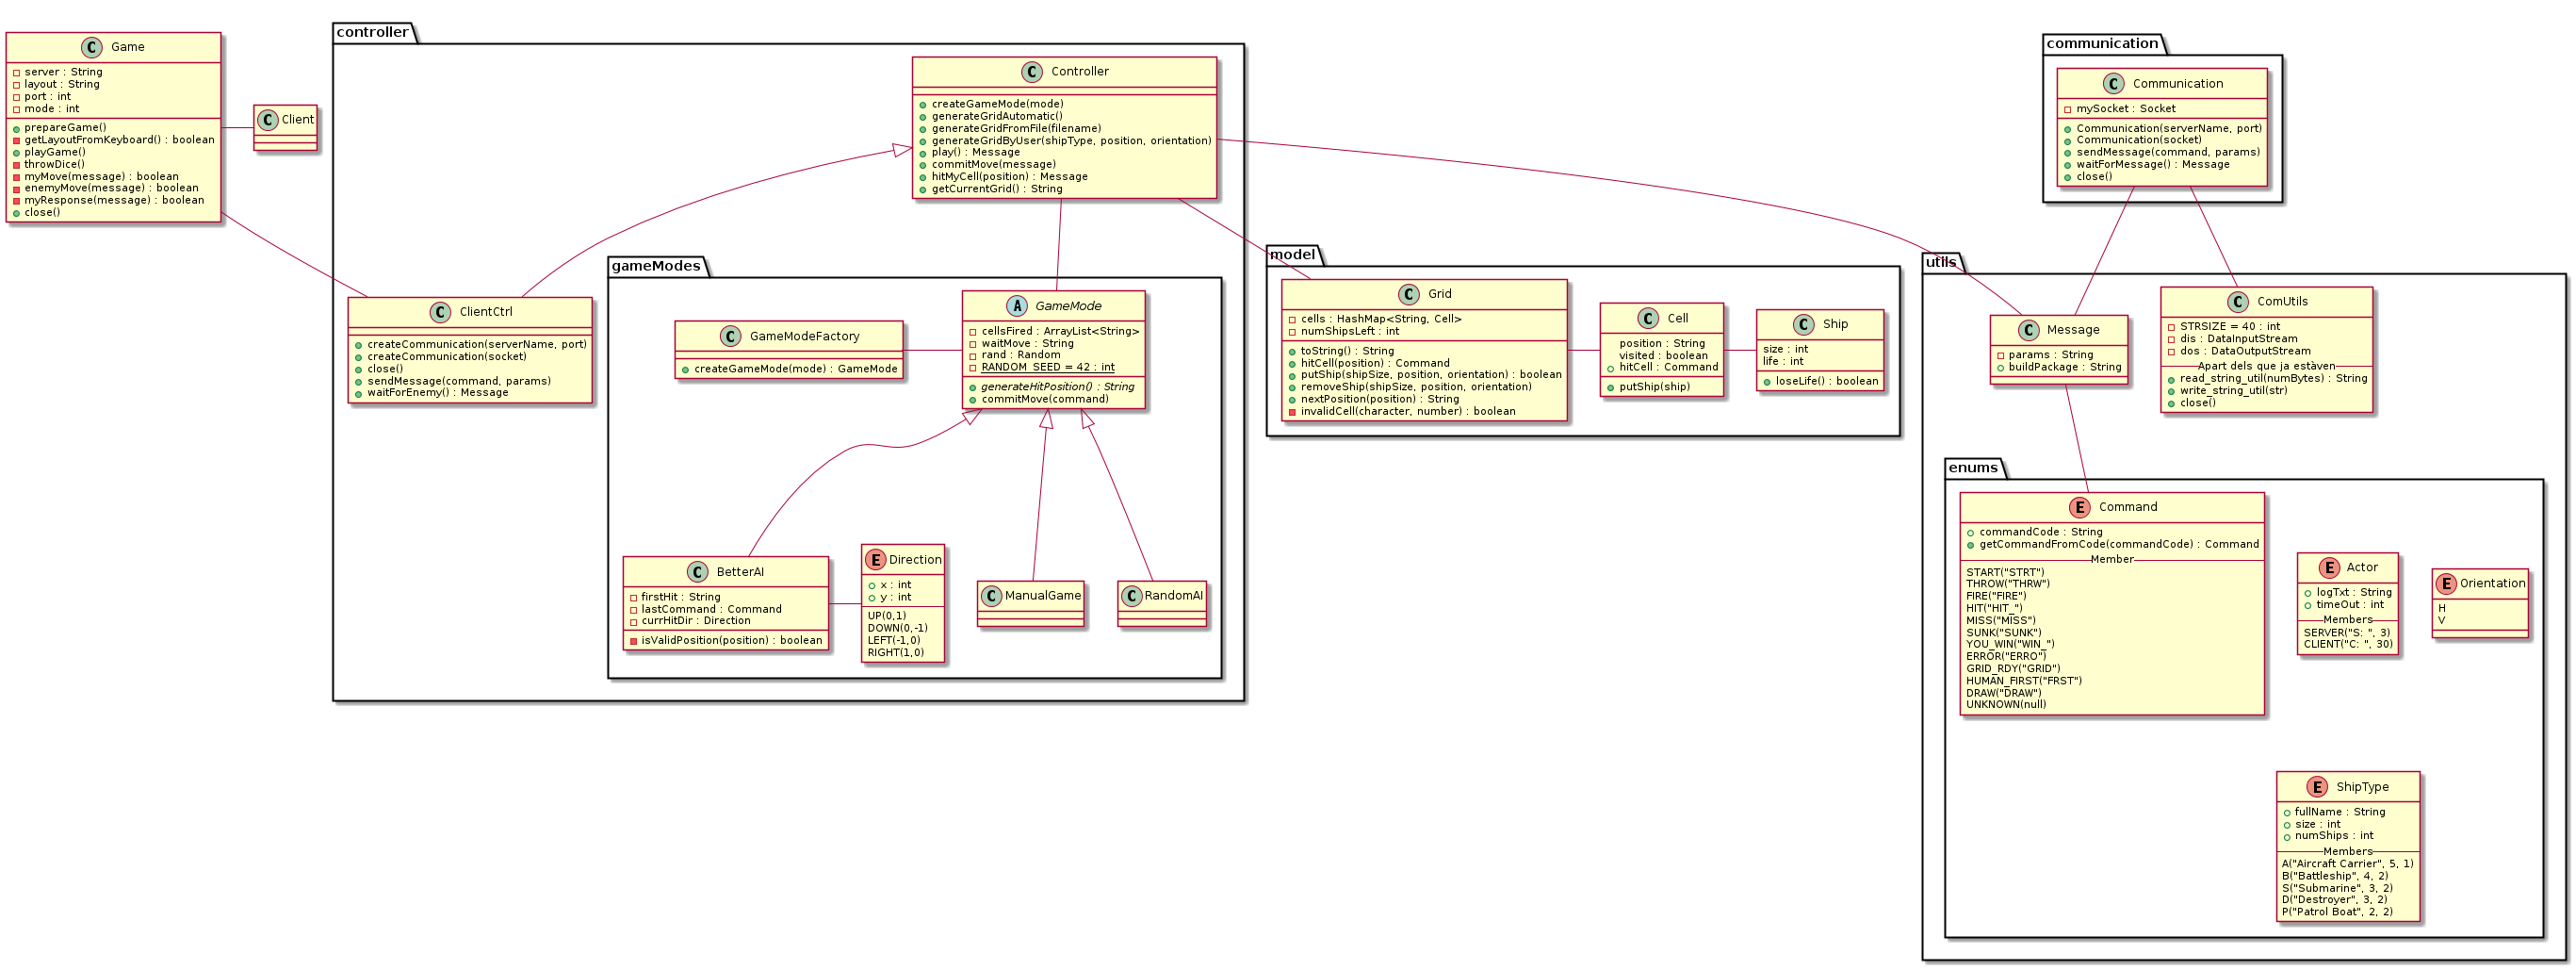
\includegraphics[width=\textwidth,height=\textheight,keepaspectratio]{../diagrams/class-diagrams/clientClasses.png}
    \caption{Client Diagram}
    \label{fig:PropProf}
\end{sidewaysfigure}
\begin{sidewaysfigure}[ht]
    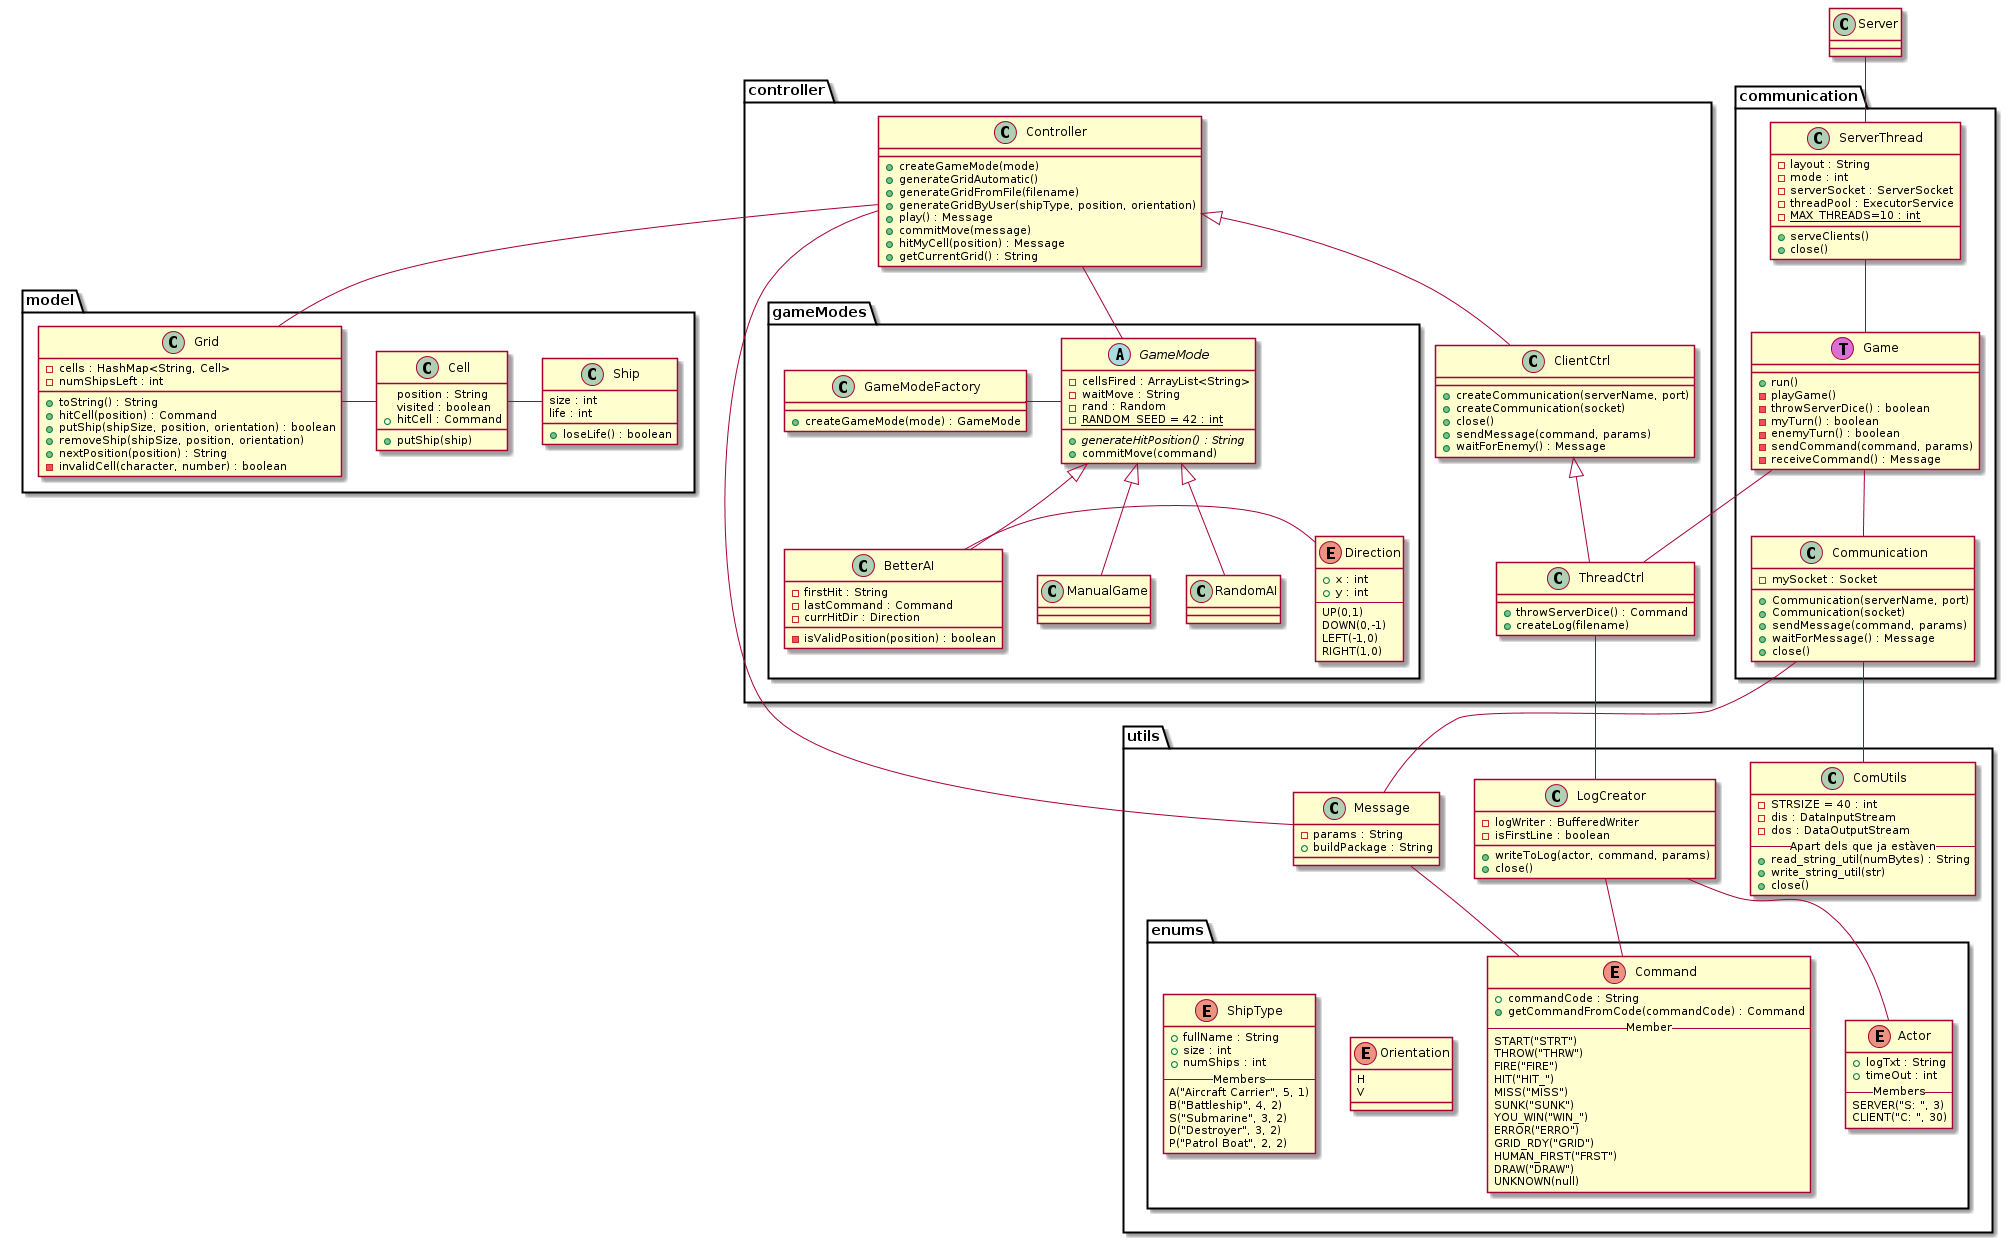
\includegraphics[width=\textwidth,height=\textheight,keepaspectratio]{../diagrams/class-diagrams/threadsClasses.png}
    \caption{Threads-Server Diagram}
    \label{fig:PropProf}
\end{sidewaysfigure}
\begin{sidewaysfigure}[ht]
    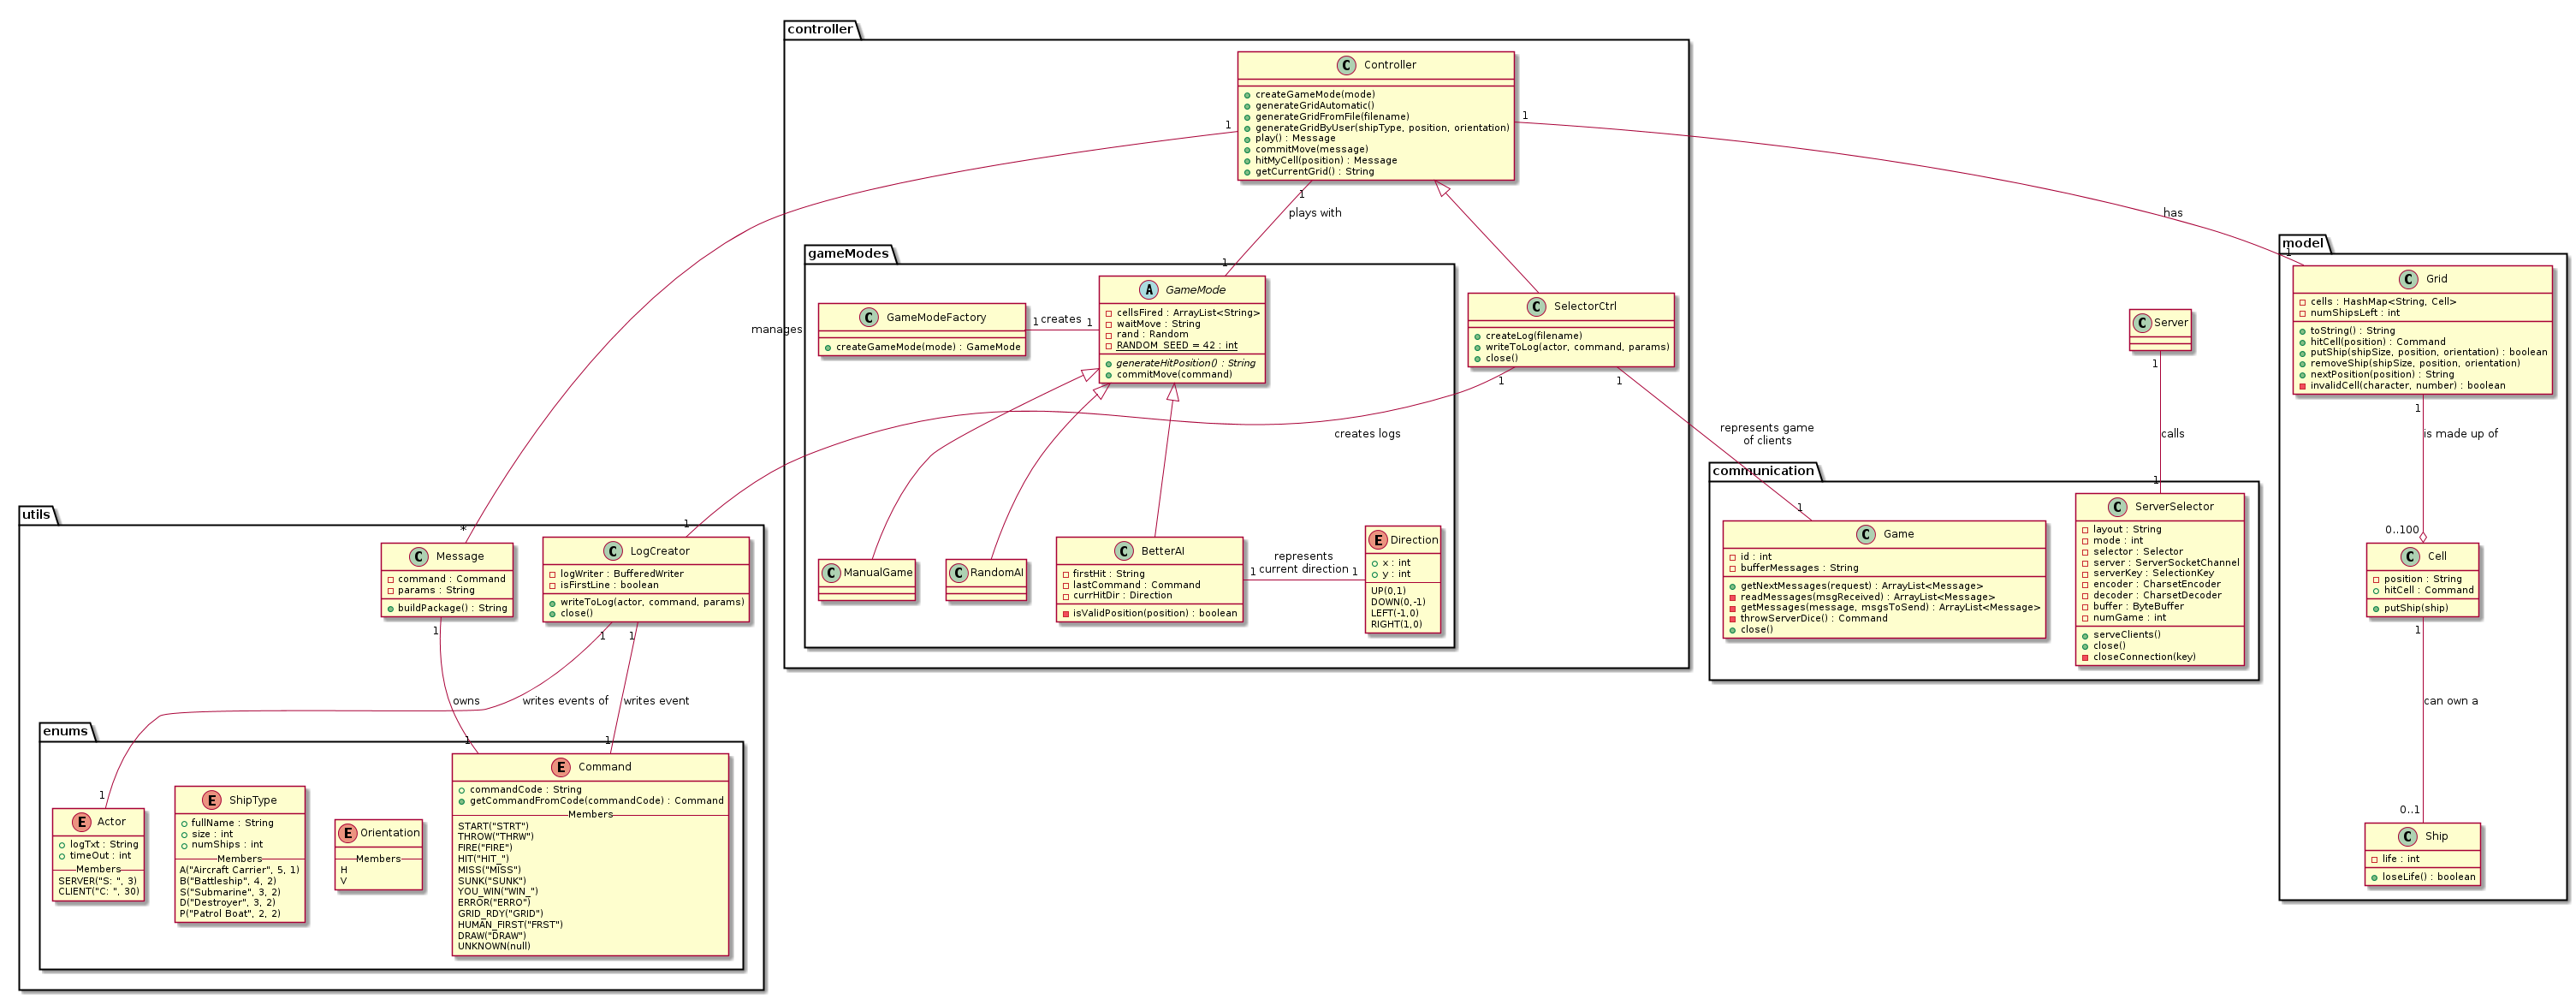
\includegraphics[width=\textwidth,height=\textheight,keepaspectratio]{../diagrams/class-diagrams/selectorClasses.png}
    \caption{Selector-Server Diagram}
    \label{fig:PropProf}
\end{sidewaysfigure}

\end{document}